\documentclass{standalone}
\usepackage{tikz}
\usetikzlibrary{patterns}
\usetikzlibrary{positioning}
\usetikzlibrary{patterns, positioning}
\usetikzlibrary{shapes.misc}
\usepackage[outline]{contour}
\contourlength{1.5pt} 
\usepackage[sfdefault]{ClearSans}

\begin{document}
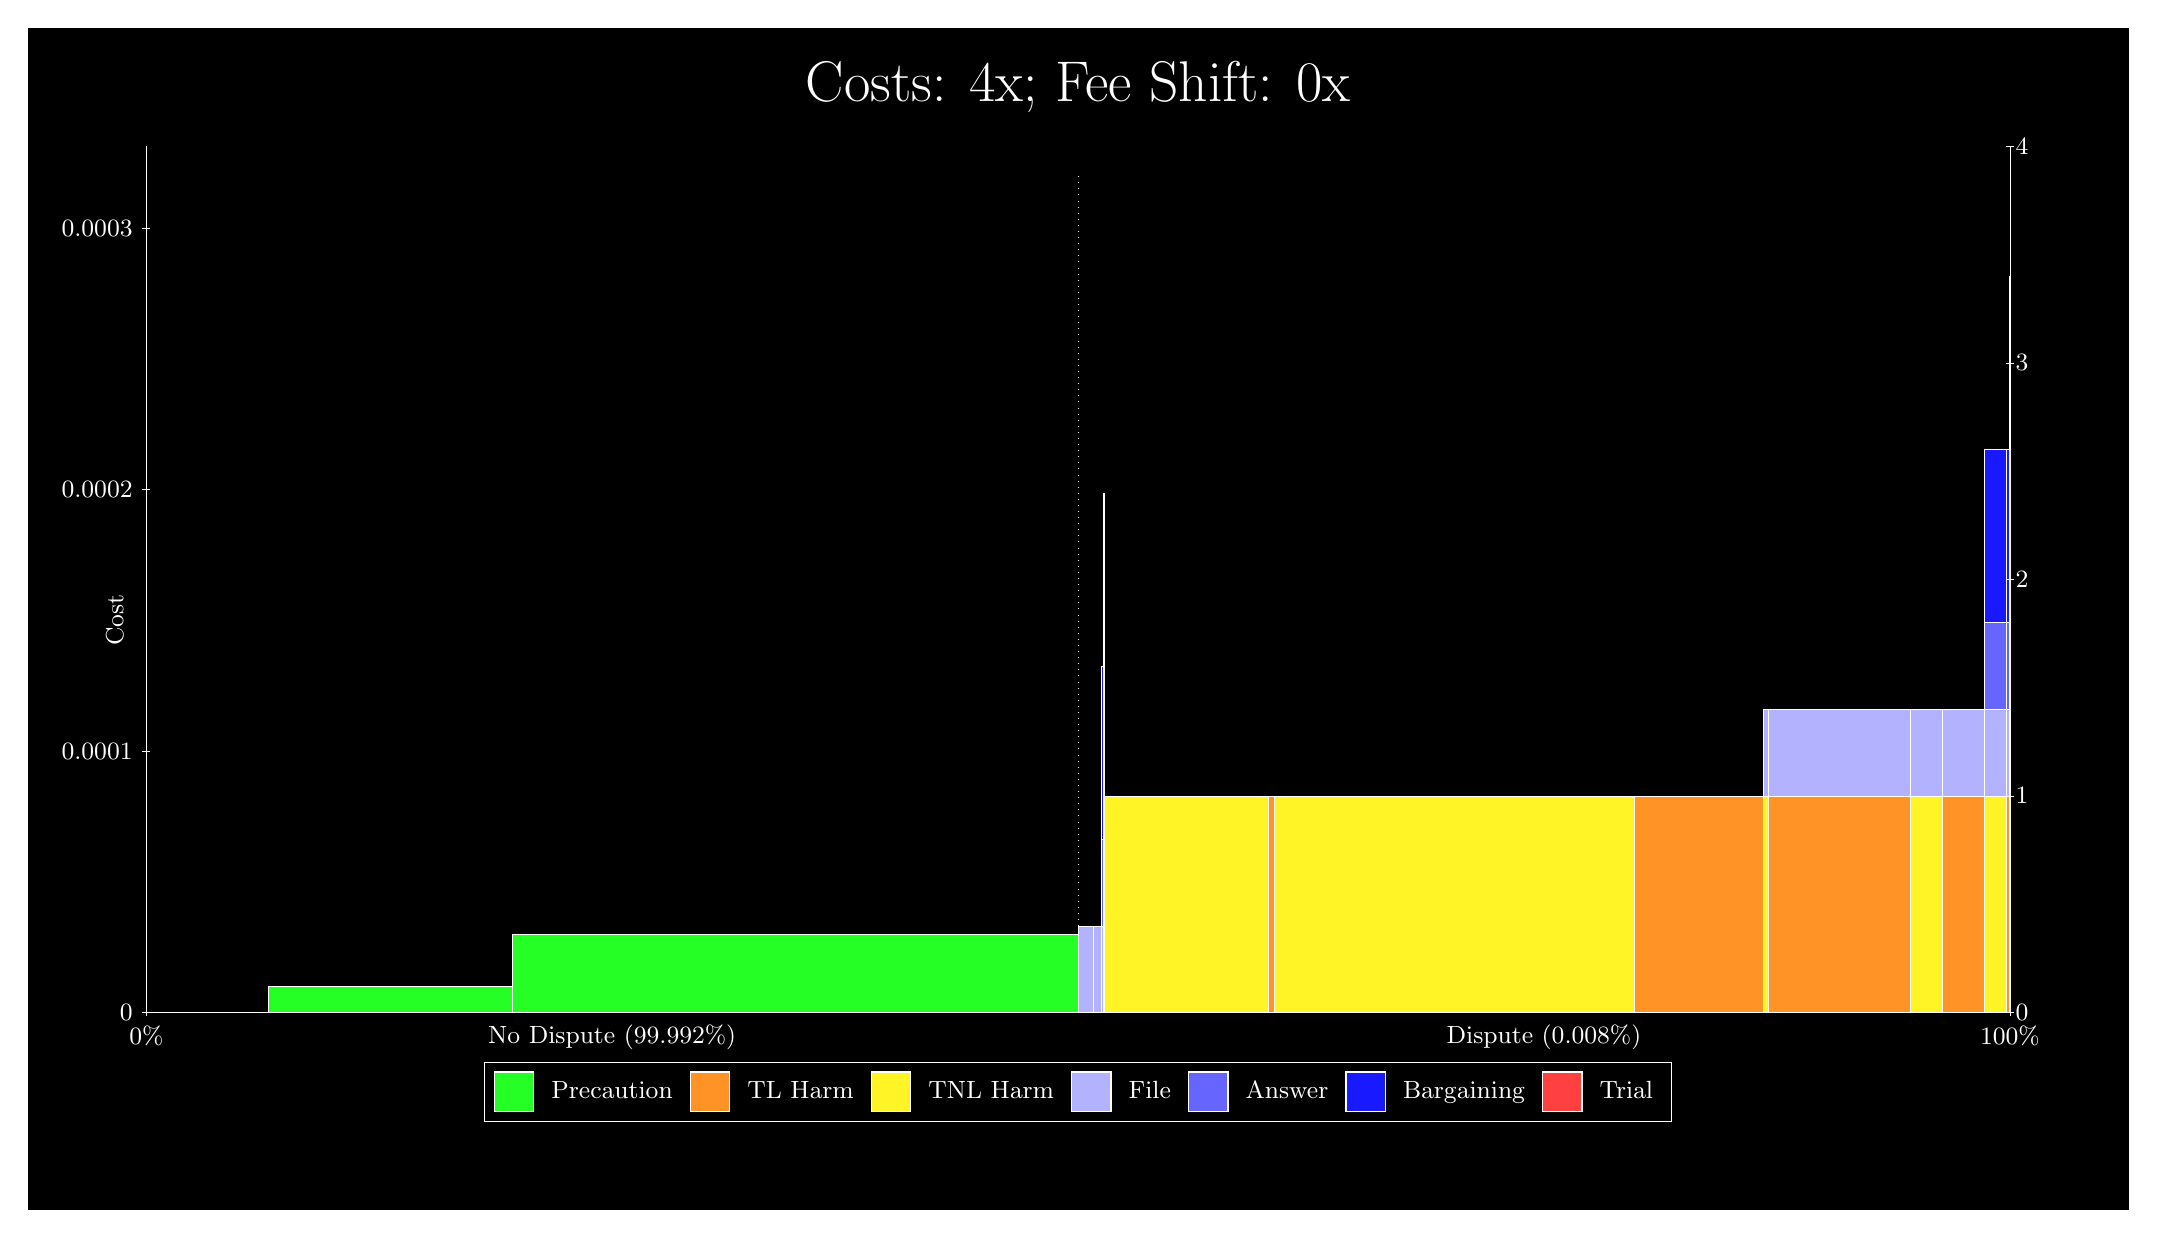
\begin{tikzpicture}
\draw[fill=black] (0,0) rectangle (26.667,15);
\draw[draw=none,text=white] (0,13.5) rectangle (26.667,15) node[midway] {\huge Costs: 4x; Fee Shift: 0x };
\draw[fill=green!85,draw=white,very thin] (3.0469,2.5) rectangle (6.144,2.832);
\draw[fill=green!85,draw=white,very thin] (6.144,2.5) rectangle (13.333,3.4961);
\draw[fill=blue!30,draw=white,very thin] (13.333,2.5) rectangle (13.52,3.6);
\draw[fill=green!85,draw=white,very thin] (13.52,2.5) rectangle (13.624,2.5);
\draw[fill=blue!30,draw=white,very thin] (13.52,2.5) rectangle (13.624,3.6);
\draw[fill=green!85,draw=white,very thin] (13.624,2.5) rectangle (13.659,2.5);
\draw[fill=blue!30,draw=white,very thin] (13.624,2.5) rectangle (13.659,3.6);
\draw[fill=blue!60,draw=white,very thin] (13.624,3.6) rectangle (13.659,4.7);
\draw[fill=blue!90,draw=white,very thin] (13.624,4.7) rectangle (13.659,6.9);
\draw[fill=green!85,draw=white,very thin] (13.659,2.5) rectangle (13.66,2.5);
\draw[fill=blue!30,draw=white,very thin] (13.659,2.5) rectangle (13.66,3.6);
\draw[fill=blue!60,draw=white,very thin] (13.659,3.6) rectangle (13.66,4.7);
\draw[fill=blue!90,draw=white,very thin] (13.659,4.7) rectangle (13.66,6.9);
\draw[fill=red!75,draw=white,very thin] (13.659,6.9) rectangle (13.66,9.1);
\draw[fill=green!85,draw=white,very thin] (13.66,2.5) rectangle (15.745,2.5);
\draw[fill=yellow!85,draw=white,very thin] (13.66,2.5) rectangle (15.745,5.25);
\draw[fill=green!85,draw=white,very thin] (15.745,2.5) rectangle (15.822,2.5);
\draw[fill=orange!85,draw=white,very thin] (15.745,2.5) rectangle (15.822,5.25);
\draw[fill=green!85,draw=white,very thin] (15.822,2.5) rectangle (20.391,2.5001);
\draw[fill=yellow!85,draw=white,very thin] (15.822,2.5001) rectangle (20.391,5.2501);
\draw[fill=green!85,draw=white,very thin] (20.391,2.5) rectangle (22.039,2.5001);
\draw[fill=orange!85,draw=white,very thin] (20.391,2.5001) rectangle (22.039,5.2501);
\draw[fill=yellow!85,draw=white,very thin] (22.039,2.5) rectangle (22.1,5.25);
\draw[fill=blue!30,draw=white,very thin] (22.039,5.25) rectangle (22.1,6.35);
\draw[fill=orange!85,draw=white,very thin] (22.1,2.5) rectangle (23.907,5.25);
\draw[fill=blue!30,draw=white,very thin] (22.1,5.25) rectangle (23.907,6.35);
\draw[fill=green!85,draw=white,very thin] (23.907,2.5) rectangle (24.312,2.5);
\draw[fill=yellow!85,draw=white,very thin] (23.907,2.5) rectangle (24.312,5.25);
\draw[fill=blue!30,draw=white,very thin] (23.907,5.25) rectangle (24.312,6.35);
\draw[fill=green!85,draw=white,very thin] (24.312,2.5) rectangle (24.841,2.5);
\draw[fill=orange!85,draw=white,very thin] (24.312,2.5) rectangle (24.841,5.25);
\draw[fill=blue!30,draw=white,very thin] (24.312,5.25) rectangle (24.841,6.35);
\draw[fill=green!85,draw=white,very thin] (24.841,2.5) rectangle (25.126,2.5);
\draw[fill=yellow!85,draw=white,very thin] (24.841,2.5) rectangle (25.126,5.25);
\draw[fill=blue!30,draw=white,very thin] (24.841,5.25) rectangle (25.126,6.35);
\draw[fill=blue!60,draw=white,very thin] (24.841,6.35) rectangle (25.126,7.45);
\draw[fill=blue!90,draw=white,very thin] (24.841,7.45) rectangle (25.126,9.65);
\draw[fill=green!85,draw=white,very thin] (25.126,2.5) rectangle (25.154,2.5);
\draw[fill=orange!85,draw=white,very thin] (25.126,2.5) rectangle (25.154,5.25);
\draw[fill=blue!30,draw=white,very thin] (25.126,5.25) rectangle (25.154,6.35);
\draw[fill=blue!60,draw=white,very thin] (25.126,6.35) rectangle (25.154,7.45);
\draw[fill=blue!90,draw=white,very thin] (25.126,7.45) rectangle (25.154,9.65);
\draw[fill=green!85,draw=white,very thin] (25.154,2.5) rectangle (25.16,2.5);
\draw[fill=yellow!85,draw=white,very thin] (25.154,2.5) rectangle (25.16,5.25);
\draw[fill=blue!30,draw=white,very thin] (25.154,5.25) rectangle (25.16,6.35);
\draw[fill=blue!60,draw=white,very thin] (25.154,6.35) rectangle (25.16,7.45);
\draw[fill=blue!90,draw=white,very thin] (25.154,7.45) rectangle (25.16,9.65);
\draw[fill=red!75,draw=white,very thin] (25.154,9.65) rectangle (25.16,11.85);
\draw[fill=green!85,draw=white,very thin] (25.16,2.5) rectangle (25.167,2.5);
\draw[fill=orange!85,draw=white,very thin] (25.16,2.5) rectangle (25.167,5.25);
\draw[fill=blue!30,draw=white,very thin] (25.16,5.25) rectangle (25.167,6.35);
\draw[fill=blue!60,draw=white,very thin] (25.16,6.35) rectangle (25.167,7.45);
\draw[fill=blue!90,draw=white,very thin] (25.16,7.45) rectangle (25.167,9.65);
\draw[fill=red!75,draw=white,very thin] (25.16,9.65) rectangle (25.167,11.85);
\draw[white,very thin] (1.5,2.5) -- (1.5,13.5);
\node[font=\small,rotate=90,text=white, anchor=center] at (1.1, 7.4803) {Cost};
\draw[white,very thin] (1.45,2.5) -- (1.55,2.5);
\node[font=\small,text=white, anchor=east] at (1.45, 2.5) {0};
\draw[white,very thin] (1.45,5.8202) -- (1.55,5.8202);
\node[font=\small,text=white, anchor=east] at (1.45, 5.8202) {0.0001};
\draw[white,very thin] (1.45,9.1404) -- (1.55,9.1404);
\node[font=\small,text=white, anchor=east] at (1.45, 9.1404) {0.0002};
\draw[white,very thin] (1.45,12.461) -- (1.55,12.461);
\node[font=\small,text=white, anchor=east] at (1.45, 12.461) {0.0003};

\draw[white,dotted,very thin] (13.333,2.83) -- (13.333,13.17);
\draw[white,very thin] (25.167,2.5) -- (25.167,13.5);
\draw[white,very thin] (25.117,2.5) -- (25.217,2.5);
\node[font=\small,text=white, anchor=west] at (25.117, 2.5) {0};
\draw[white,very thin] (25.117,5.25) -- (25.217,5.25);
\node[font=\small,text=white, anchor=west] at (25.117, 5.25) {1};
\draw[white,very thin] (25.117,8) -- (25.217,8);
\node[font=\small,text=white, anchor=west] at (25.117, 8) {2};
\draw[white,very thin] (25.117,10.75) -- (25.217,10.75);
\node[font=\small,text=white, anchor=west] at (25.117, 10.75) {3};
\draw[white,very thin] (25.117,13.5) -- (25.217,13.5);
\node[font=\small,text=white, anchor=west] at (25.117, 13.5) {4};

\draw[white,very thin] (1.5,2.5) -- (25.167,2.5);
\draw[white,very thin] (1.5,2.45) -- (1.5,2.55);
\node[font=\small,text=white, anchor=north] at (1.5, 2.45) {0\%};
\draw[white,very thin] (25.167,2.45) -- (25.167,2.55);
\node[font=\small,text=white, anchor=north] at (25.167, 2.45) {100\%};

\node[font=\small,text=white,anchor=south] at (7.4167, 1.9) {No\ Dispute\ (99.992\%)};
\node[font=\small,text=white,anchor=south] at (19.25, 1.9) {Dispute\ (0.008\%)};
\draw (13.3333,2.5) node (B) {};
\begin{scope}[align=center]
\matrix[scale=0.5,draw=white,below=0.5cm of B,nodes={draw},column sep=0.1cm]{
\node[rectangle,draw,minimum width=0.5cm,minimum height=0.5cm,fill=green!85]{}; & \node[draw=none,font=\small,text=white]{Precaution}; &
\node[rectangle,draw,minimum width=0.5cm,minimum height=0.5cm,fill=orange!85]{}; & \node[draw=none,font=\small,text=white]{TL Harm}; &
\node[rectangle,draw,minimum width=0.5cm,minimum height=0.5cm,fill=yellow!85]{}; & \node[draw=none,font=\small,text=white]{TNL Harm}; &
\node[rectangle,draw,minimum width=0.5cm,minimum height=0.5cm,fill=blue!30]{}; & \node[draw=none,font=\small,text=white]{File}; &
\node[rectangle,draw,minimum width=0.5cm,minimum height=0.5cm,fill=blue!60]{}; & \node[draw=none,font=\small,text=white]{Answer}; &
\node[rectangle,draw,minimum width=0.5cm,minimum height=0.5cm,fill=blue!90]{}; & \node[draw=none,font=\small,text=white]{Bargaining}; &
\node[rectangle,draw,minimum width=0.5cm,minimum height=0.5cm,fill=red!75]{}; & \node[draw=none,font=\small,text=white]{Trial}; \\\\
};\end{scope}

\end{tikzpicture}
\end{document}